\chapter{Limitations and constraints}
In the course of our project, we were faced with several limitations and constraints that influenced our progress and our ability to achieve our objectives. These challenges added further complexity to our work and required proactive management to overcome them.\\

\subsection{The robot}
First of all, the lack of resources available online to solve the specific problems we encountered with the QTrobot was a big obstacle. Indeed, there is very little help or documentation available to guide us. This meant that our learning curve was slowed down enormously, as we had to spend a lot of time searching for relevant information and solving problems by trial and error.\\
\\
\\
\begin{minipage}{.65\textwidth}%
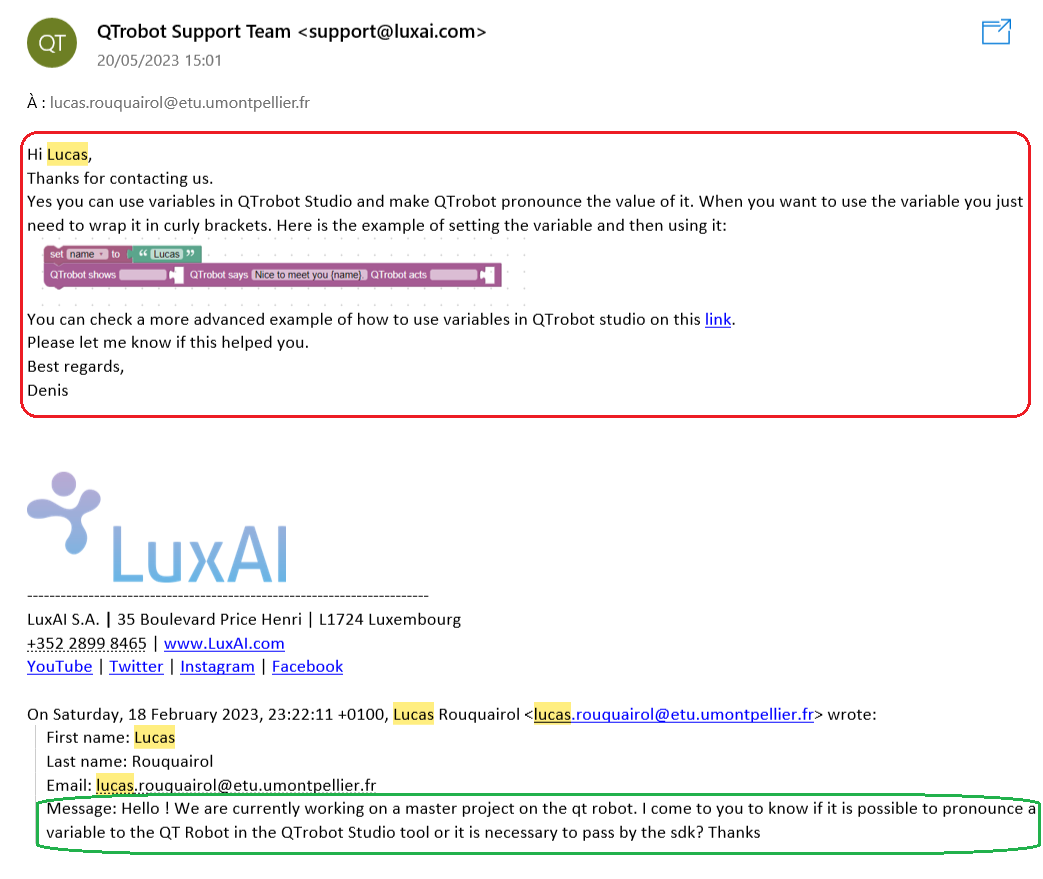
\includegraphics[width=\textwidth]{Figures/qtsupportemail.png}
\captionof{figure}{Exchange with support}
\end{minipage}%
\hfill
\begin{minipage}{.33\textwidth}%
When we encountered more complex problems, we had to call on technical support via e-mail. Unfortunately, support response times were sometimes slow, resulting in further delays in resolving our problems. We had to manage our impatience while continuing to work autonomously wherever possible.\\
\end{minipage}%
\newpage
In addition, limited access to the robot was a major obstacle. The robot was stored in the secretariat of Building 16, which meant that it could only be accessed during the secretariat's opening hours, i.e. only on weekdays and before 5pm. What's more, as other teams also had to use it, we had to plan our usage time carefully. These constraints led to delays in our development schedule and limited our scope for experimentation. We had to organize ourselves efficiently to optimize every moment of access to the robot.\\
\\
\subsection{The time}
The partial availability of our team was a constant challenge. Indeed, due to various constraints, not all team members were available simultaneously. This complicated coordination and collaboration within the group, sometimes resulting in additional delays and uneven distribution of tasks.\\
\\
What's more, we were under considerable time pressure. We had to finalize the project quickly in order to present it to the participants. This put additional pressure on the team, limiting our ability to make in-depth improvements or explore advanced QTrobot functionalities. We had to focus on the essentials to meet the deadline.\\
\\
\subsection{The experience}
Finally, the difficulty of bringing together all the participants in the experiment on the same day was a major challenge to ensuring effective communication and collaboration. Constraints related to individual availability led to delays and absences of some participants, which had a direct impact on the overall progress of the project. To overcome this situation, we had to maintain constant coordination and make frequent adjustments to the schedule. We had to be flexible and responsive in order to find time slots that suited all participants, and this required careful management of everyone's schedules. Despite these logistical challenges, we maintained an open and regular dialogue with all participants, ensuring that everyone was informed of developments and could actively contribute to the experience.\\
\\
